We evaluate the efficacy of Roots as a performance monitoring and root cause
analysis system for PaaS applications.
To do so, we consider its ability to identify and characterize SLO violations.
For violations that are not caused by a change in workload, we evaluate Roots' ability to identify
the PaaS component that is the cause of the performance anomaly. We also
evaluate the Roots path distribution analyzer, and its ability to identify
execution paths along with changes in path distributions.
Finally, we investigate the performance and scalability of the Roots
prototype. 

\subsection{Anomaly Detection: Accuracy and Speed}

\begin{table}
\begin{center}
\begin{tabular}{|c|p{2cm}|p{2cm}|p{2cm}|}
\hline
Faulty Service & $L_1$ (30ms) & $L_2$ (35ms) & $L_3$ (45ms) \\ \hline
datastore & 18 & 11 & 10 \\ \hline
user management & 19 & 15 & 10 \\ \hline
\end{tabular}
\end{center}
\caption{Number of anomalies detected in guestbook app under different SLOs 
($L_1$, $L_2$ and $L_3$) when injecting faults into two different PaaS kernel services.
\label{tab:anomaly_counts}
}
\end{table}

To begin the evaluation of the Roots prototype we experiment with
the SLO-based anomaly detector, using a simple HTML-producing Java 
web application called ``guestbook''.
This application allows users to login, and post comments. It uses the
AppScale  datastore service to save
the posted comments, and the AppScale user management service to handle authentication. Each request processed
by guestbook results in two PaaS kernel invocations -- one to check if the user is logged in, and 
another to retrieve the existing comments from the datastore. We conduct all
our experiments on a single node AppScale cloud except where specified. The node itself is an Ubuntu
14.04 VM with 4 virtual CPU cores (clocked at 2.4GHz), and 4GB of memory.

We run the SLO-based anomaly detector on guestbook with a sampling rate of 15 seconds, an analysis
rate of 60 seconds, and a window size of 1 hour. We set the minimum sample count to 100, and
run a series of experiments with different SLOs on the guestbook application. Specifically, we fix
the SLO success probability at 95\%, and set the response time upper bound to $\mu_g + n\sigma_g$. 
$\mu_g$ and $\sigma_g$ represent the mean and standard deviation of the
guestbook's response time. We learn these two parameters apriori by benchmarking
the application. Then we obtain three different upper bound values for the guestbook's
response time by setting 
$n$ to 2, 3 and 5. We denote the resulting three SLOs $L_1$, $L_2$ and $L_3$ respectively.

We also inject performance faults into AppScale by modifying its code
to cause the datastore service to be slow to respond.
This fault injection logic activates once every hour, and
slows down all datastore invocations by 45ms over a period of 3 minutes.
We chose 45ms because it is equal 
to $\mu_g + 5\sigma_g$ for the guestbook deployment under test. 
Therefore this delay is sufficient to violate all three SLOs used in our experiments. 
We run a similar set of experiments where we inject faults into the user management service of
AppScale. Each experiment is run for a period of 10 hours.

Table~\ref{tab:anomaly_counts} shows how the number of anomalies detected by 
Roots in a 10 hour period varies when the SLO is changed. The number of anomalies
drops noticeably when the response time upper bound is increased. When the $L_3$
SLO (45ms) is used, the only anomalies detected are the ones
caused by our hourly fault injection mechanism. As the SLO is tightened by lowering the upper bound,
Roots detects additional anomalies. These additional anomalies
result from a combination of injected faults, and other naturally occurring faults
in the system. That is, Roots detected some naturally occurring
faults (temporary spikes in application latency), when a number of injected faults
were still in the sliding window of the anomaly detector. Together these two types of
faults caused SLO violations, usually several minutes after the fault injection period
has expired.

Next we analyze how fast Roots can detect anomalies in an application. We
first consider the performance of guestbook under the $L_1$ SLO while 
injecting faults into the datastore service. Figure~\ref{fig:time_line_guestbook_2s} shows
anomalies detected by Roots as events on a time line. The horizontal axis represents 
passage of time. The red arrows indicate the start of a fault injection period, where each
period lasts up to 3 minutes.
The blue arrows indicate the Roots anomaly detection events.
Note that every fault injection period is immediately followed by an anomaly
detection event, implying near real time reaction from Roots, except in case of the fault
injection window at 20:00 hours. Roots detected a naturally occurring anomaly
(i.e. one
that we did not explicitly inject, but nonetheless caused an SLO violation) at 19:52 hours,
which caused the anomaly detector to go into the warm up mode. Therefore Roots
did not immediately react to the faults injected at 20:00 hours. But as soon as the detector became
active again at 20:17, it detected the anomaly.

\begin{figure}
\centering
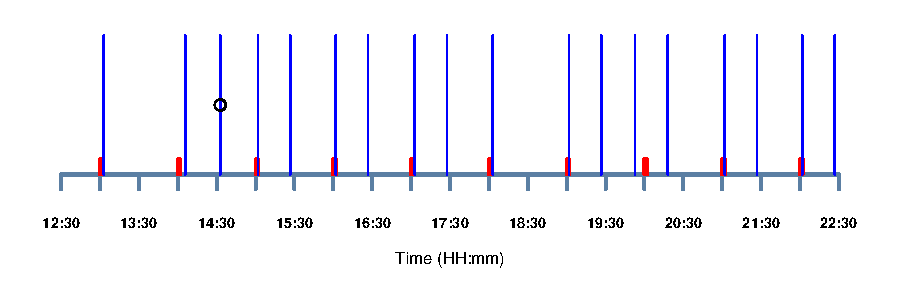
\includegraphics[scale=0.65]{time_line_guestbook_2s}
\caption{Anomaly detection in guestbook application during a period of 10 hours. Red arrows indicate fault injection 
at the datastore service. Blue arrows indicate all anomalies detected by Roots during the experimental run.}
\label{fig:time_line_guestbook_2s}
\end{figure}

\begin{figure}
\centering
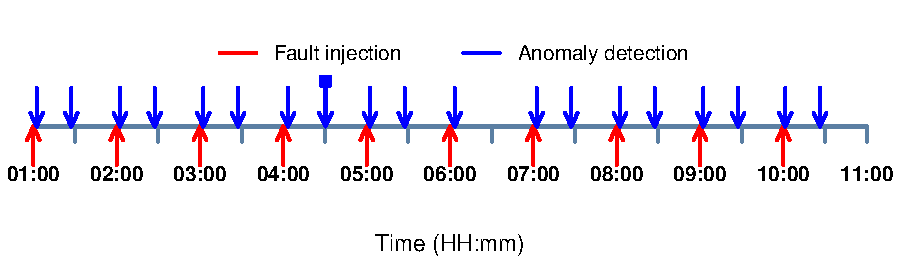
\includegraphics[scale=0.65]{time_line_guestbook_2s_user}
\caption{Anomaly detection in guestbook application during a period of 10 hours. Red arrows indicate fault injection
at the user management service. Blue arrows indicate all anomalies detected by Roots during the experimental run.}
\label{fig:time_line_guestbook_2s_user}
\end{figure}

Figure~\ref{fig:time_line_guestbook_2s_user} shows the anomaly detection time line for the 
same application and SLO, while faults are being injected into the user management service.
Here too we see that Roots detects anomalies immediately following each fault injection window.

%All the results discussed up to this point
%demonstrate the efficacy of our anomaly detection method. The SLO-based
%anomaly detector used in Roots is correct by construction, in the sense it simply detects whenever
%an application fails to uphold a preconfigured performance SLO. Since each SLO violation is caused
%by an unexpected performance degradation in the application, Roots can be expected to correctly identify
%performance anomalies via the observed SLO violations.

\subsection{Path Distribution Analyzer: Accuracy and Speed}
\begin{figure}
\centering
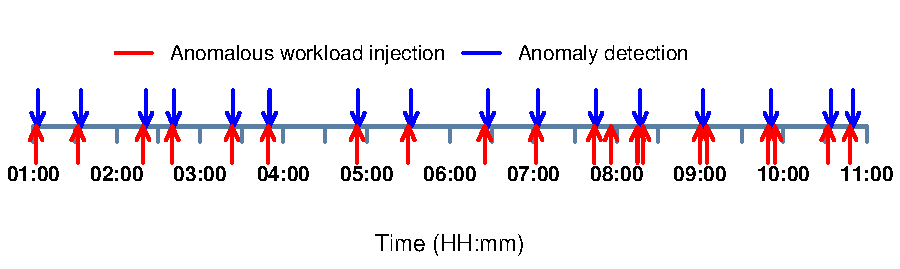
\includegraphics[scale=0.65]{time_line_crud}
\caption{Anomaly detection in key-value store application during a period of 10 hours. Steady-state traffic is read-heavy. Red arrows
indicate injection of write-heavy bursts. Blue arrows indicate all the anomalies detected by the path distribution
analyzer.}
\label{fig:time_line_crud}
\end{figure}

\begin{figure}
\centering
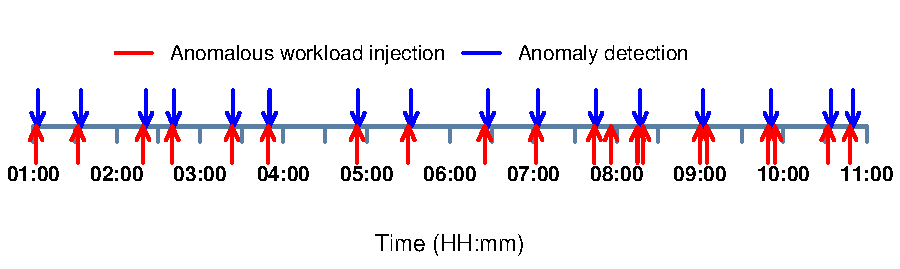
\includegraphics[scale=0.65]{time_line_caching}
\caption{Anomaly detection in cached key-value store application during a period of 10 hours. Steady-state traffic is mostly
served from the cache. Red arrows
indicate injection of cache-miss bursts. Blue arrows indicate all the anomalies detected by the path distribution
analyzer.}
\label{fig:time_line_caching}
\end{figure}

Next we evaluate the effectiveness and accuracy of the path distribution analyzer. For this we 
employ two different applications.
\begin{description}
\item[key-value store] This application provides the functionality of an online key-value store.  It allows 
users to store data objects in the cloud where each object is assigned a unique key. The objects can then be 
retrieved, updated or deleted using their keys. Different operations
(create, retrieve, update and delete) are implemented as separate paths of
execution in the application.
\item[cached key-value store] This is a simple extension of the regular key-value store, which adds
caching to the read operation using the AppScale's memcache service. The application contains
separate paths of execution for cache hits and cache misses.
\end{description}

We first deploy the key-value store on AppScale, and populate it with a number of data objects. Then we
run a test client against it which generates a read-heavy workload. On average this workload
consists of 90\% read requests and 10\% write requests. The test client
is also programmed to randomly send bursts of write-heavy workloads. These bursts consist
of 90\% write requests on average, and each burst lasts up to 2 minutes. Figure~\ref{fig:time_line_crud}
shows the write-heavy bursts as events on a time line (indicated by red arrows). Note that almost every burst is
immediately followed by an anomaly detection event (indicated by blue arrows). 
The only time we do not see an anomaly detection event is when multiple
bursts are clustered together in time (e.g. 3 bursts between 17:04 and 17:24 hours). In this
case Roots detects the very first burst, and then goes into the warm up mode to collect more data. 
Between 20:30 and 21:00 hours we also
had two instances where the read request proportion dropped from 90\% to 80\% due to random
chance. 
This is because our test client randomizes the read request proportion around the 90\% mark. 
Roots identified these two incidents also as anomalous.

We conduct a similar experiment using the cached key-value store. Here, we run a test client that generates a workload
that is mostly served from the cache. This is done by repeatedly executing read requests on a small
selected set of object keys. However, the client randomly sends bursts of traffic requesting keys that
are not likely to be in the application cache, thus resulting in many cache misses. Each burst
lasts up to 2 minutes. As shown in 
figure~\ref{fig:time_line_caching}, Roots path distribution analyzer correctly detects the change 
in the workload (from many cache hits to many cache misses), nearly every time the test client injects a 
burst of traffic that triggers the cache miss path of the application. The only exception is when
multiple bursts are clumped together, in which case only the first raises an alarm in Roots.

\subsection{Workload Change Analyzer Accuracy}
\begin{figure}
\centering
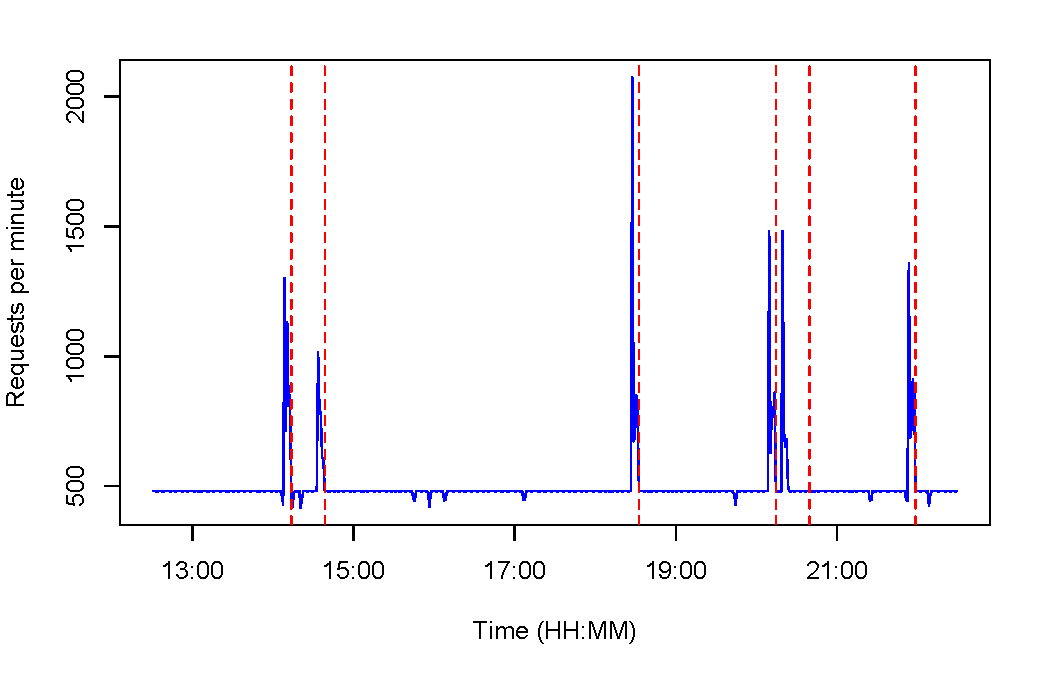
\includegraphics[scale=0.5]{workload_change_trace}
\caption{Workload size over time for the key-value store application. The test client randomly sends
large bursts of traffic causing the spikes in the plot. Roots anomaly detection events are shown
in red dashed lines.}
\label{fig:workload_change}
\end{figure}

Next we evaluate the Roots workload change analyzer. In this experiment we run a varying workload
against the key-value store application for 10 hours. The load generating client is programmed
to maintain a mean workload level of 500 requests per minute. However, the client
is also programmed to randomly send large bursts of traffic at times of its choosing. During these bursts 
the client may send more than 1000 requests a minute, thus impacting the performance of
the application server that hosts the key-value store. Figure~\ref{fig:workload_change} shows how
the application workload has changed over time. The workload generator has produced 6 large bursts of traffic during the 
period of the experiment, which appear as tall spikes in the plot.
Note that each burst is immediately followed by a Roots anomaly detection event (shown by red dashed lines). 
In each of these 6 cases, the increase in workload caused a violation of the application performance SLO.
Roots detected the corresponding anomalies, and determined them to be caused by changes in the workload size.
As a result, bottleneck identification was not triggered for any of these anomalies.
Even though the bursts of traffic appear to be momentary
spikes, each burst lasts for 4 to 5 minutes thereby causing a lasting impact on the application performance.
%The PELT change point detection method used in this experimental set up is ideally suited for detecting
%such lasting changes in the workload level.

\subsection{Bottleneck Identification Accuracy}
Next we evaluate the bottleneck identification capability of Roots. We first discuss the results obtained using
the guestbook application, and follow with
results obtained using a more complex application.
In the experimental run illustrated in 
figure~\ref{fig:time_line_guestbook_2s}, Roots determined that all the detected anomalies except for one were 
caused by the AppScale datastore service. This is consistent with our expectations since in this experiment we 
artificially inject faults into the datastore. 
The only anomaly that is not traced back to the datastore service is the one that was detected at 14:32 hours.
This is indicated by the blue arrow with a small square marker at the top. For this anomaly, Roots concluded that
the bottleneck is the local execution at the application server ($r$). We have verified
this result by manually inspecting the AppScale logs, and traces of data collected by Roots. As it turns out,
between 14:19 and
14:22 the application server hosting the guestbook application experienced some problems, which caused
request latency to increase significantly. 
Therefore we can conclude that Roots has correctly identified 
the root causes of all 18 anomalies in this experimental run
including one that we did not inject explicitly. 

Similarly, in the experiment shown in figure~\ref{fig:time_line_guestbook_2s_user}, Roots determined
that all the anomalies are caused by the user management service, except in one instance. This is again
inline with our expectations since in this experiment we inject faults into the user management service. For the
anomaly detected at 04:30 hours, Roots determined that local execution time is the primary bottleneck.
Like earlier, we have manually verified this diagnosis to be accurate.
In this case too the server hosting the guestbook application became slow
during the 04:23 - 04:25 time window, and Roots correctly identified the bottleneck as the local
application server.

\begin{figure}
\centering
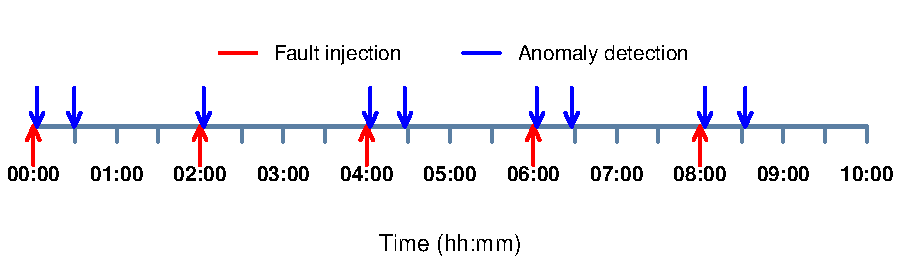
\includegraphics[scale=0.65]{time_line_stocks_1}
\caption{Anomaly detection in stock-trader application during a period of 10 hours. Red arrows indicate fault injection
at the 1st datastore query. Blue arrows indicate all anomalies detected by Roots during the experimental run.}
\label{fig:time_line_stocks_1}
\end{figure}

\begin{figure}
\centering
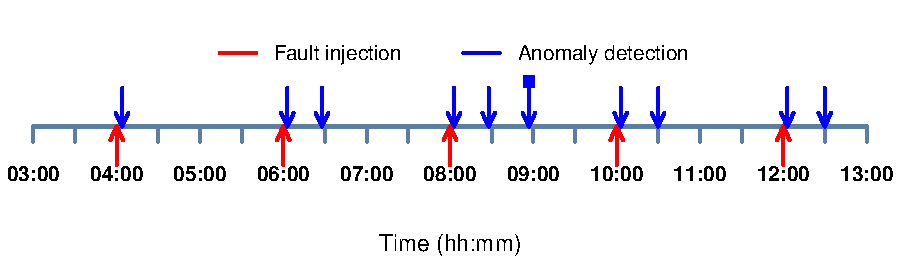
\includegraphics[scale=0.65]{time_line_stocks_2}
\caption{Anomaly detection in stock-trader application during a period of 10 hours. Red arrows indicate fault injection
at the 2nd datastore query. Blue arrows indicate all anomalies detected by Roots during the experimental run.}
\label{fig:time_line_stocks_2}
\end{figure}

In order to evaluate how the bottleneck identification performs when an application makes more than 2
PaaS kernel invocations, we conduct another experiment using an application
called ``stock-trader''.
This application allows setting up organizations, and simulating trading of stocks between the
organizations. The two main operations in this application are \textit{buy} and \textit{sell}. Each of
these operations makes 8 calls to the AppScale datastore. 
According to our previous work~\cite{Jayathilaka:2015:RTS:2806777.2806842}, 8 kernel invocations in the
same path of execution is very rare in web applications developed for a PaaS cloud. The probability
of finding an execution path with more than 5 kernel invocations in a sample of PaaS-hosted
applications is less than 1\%. Therefore the stock-trader application is a good extreme case
example to test the Roots bottleneck identification support.
We execute a number of experimental runs using this application,
and here we present the results from two of them. In all experiments we configure the anomaly
detector to check for the response time SLO of 177ms with 95\% success probability.

In one of our experimental runs we inject faults into the first datastore query executed by the buy operation
of stock-trader. The fault injection logic runs every two hours, and lasts for 3 minutes. The duration of
the full experiment is 10 hours. 
Figure~\ref{fig:time_line_stocks_1} shows the resulting event sequence. Note that every fault injection
event is immediately followed by a Roots anomaly detection event. There are also four additional
anomalies in the time line which were SLO violations caused by a combination of injected faults, and
naturally occurring faults in the system. For all the anomalies detected
in this test, Roots correctly selected the first datastore call in the application code as the bottleneck. 
The additional four anomalies occurred when a large number of injected faults were still in the sliding window
of the detector. Therefore, it is accurate to attribute those anomalies also to the first datastore query
of the application.

Figure~\ref{fig:time_line_stocks_2} shows the results from a similar experiment where we inject
faults into the second datastore query executed by the operation. Here also Roots detects all the
artificially induced anomalies along with a few extras. All the anomalies, except for one, 
are determined to be caused by the second
datastore query of the buy operation. The anomaly detected at 08:56 (marked with a square on top of the blue arrow) 
is attributed to the fourth datastore query executed by the application. We have manually verified this
diagnosis to be accurate. 
Since 08:27, when the previous anomaly was detected, the fourth datastore
query has frequently taken a long time to execute (again, on
its own), which resulted in an SLO violation at 08:56 hours.

In the experiments illustrated in figures~\ref{fig:time_line_guestbook_2s}, \ref{fig:time_line_guestbook_2s_user}, 
\ref{fig:time_line_stocks_1}, and \ref{fig:time_line_stocks_2} we maintain
the application request rate steady throughout the 10 hour periods. Therefore,
the workload change analyzer of Roots did not detect any significant shifts in the workload level. 
Consequently, none of the anomalies detected in these 4 experiments were attributed to a workload change.
The bottleneck identification was therefore triggered for each anomaly.

To evaluate the agreement level among the four bottleneck candidate selection methods, we analyze 407
anomalies detected by Roots over a period of 3 weeks. We report that except on 13 instances, in all the 
remaining cases 2 or more candidate selection methods agreed on the final bottleneck component chosen.
This implies that most of the time (96.8\%) Roots 
identifies bottlenecks with high confidence.

%\begin{figure}
%\centering
%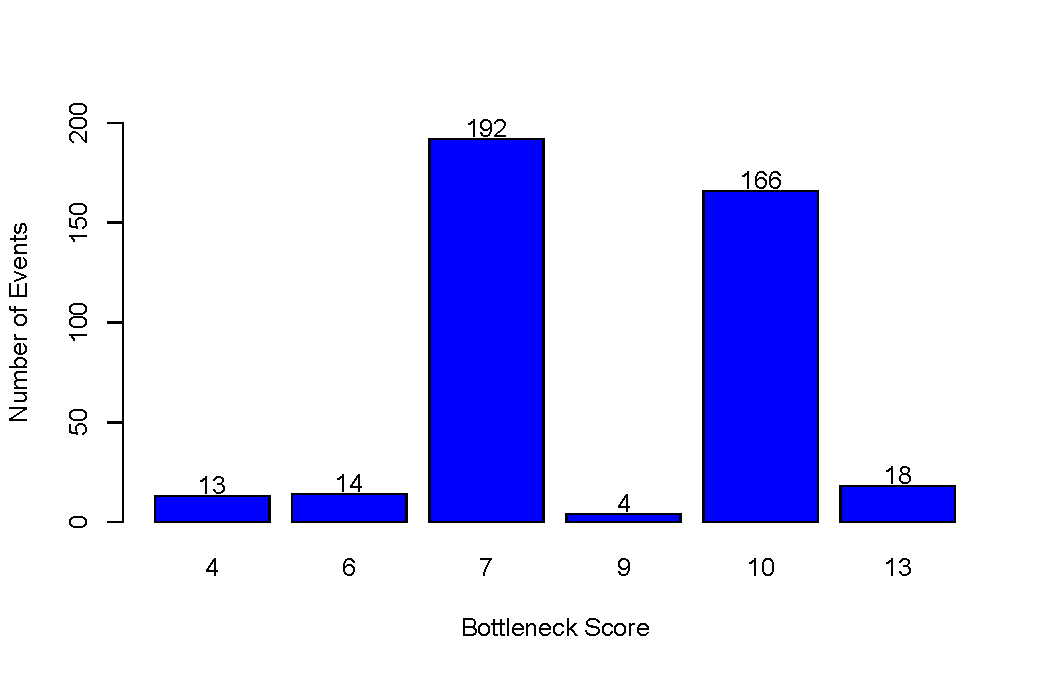
\includegraphics[scale=0.5]{bottleneck_scores}
%\caption{Frequency of different bottleneck scores.}
%\label{fig:bottleneck_scores}
%\end{figure}

%Recall that the bottleneck identification algorithm in Roots
%selects up to four candidate components for each performance anomaly detected, and then ranks them
%by assigning scores to identify the most likely bottleneck. Figure~\ref{fig:bottleneck_scores} shows the breakdown of 407 anomalies
%detected over a period of 3 weeks. X-axis represents the different scores given to candidate components
%by our algorithm. Y-axis shows the number of times a particular score was the highest. 
%According to this result, on 13 occasions Roots determined the bottleneck based on the highest score
%of 4 (score given to the component identified by the relative importance metric). 
%This happens when the algorithm chooses four different candidates
%for the bottleneck. However, this constitutes only 3.2\% of all the anomalies. In 96.8\% of the time Roots saw
%at least two of the four candidates to be the same (score values 6 or higher). This implies that most of the time Roots is able to
%identify bottlenecks with a high level of confidence since two or more candidate detection methods
%agree on their results.

\subsection{Multiple Applications in a Clustered Setting}
\begin{figure}
\centering
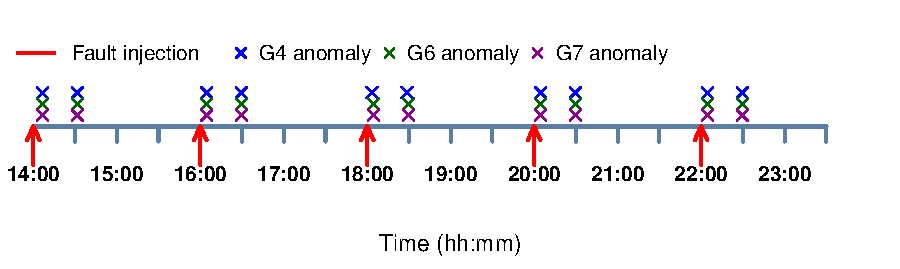
\includegraphics[scale=0.65]{time_line_g1g8}
\caption{Anomaly detection in 8 applications deployed in a clustered AppScale cloud. Red arrows
indicate fault injection at the datastore service for queries generated from a specific host. Cross
marks indicate all the anomalies detected by Roots during the experiment.}
\label{fig:time_line_g1g8}
\end{figure}

%So far we have been experimenting with a simple AppScale cloud deployed on a single virtual machine.
To demonstrate how Roots can be used in a multi-node environment, we set up an AppScale cloud
on a cluster of 10 virtual machines (VMs). VMs are provisioned by a Eucalyptus (IaaS)
cloud, and each VM is comprised of 2 CPU cores and 2GB memory. Then we proceed
to deploy 8 instances of the guestbook application on AppScale. We use the multitenant support
in AppScale to register each instance of guestbook as a different application (named $G1$ through $G8$). 
Each instance
is hosted on a separate application server instance, has its own private namespace on the AppScale
datastore, and can be accessed via a unique URL. We disable auto-scaling support in 
the AppScale cloud, and inject faults into the datastore service of AppScale in such a way that queries
issued from a particular VM, are processed with a 100ms delay. We identify this VM by its IP address
in our test environment, and shall refer to it as $V_f$ in the discussion. We trigger
the fault injection every 2 hours, and when activated it lasts for up to 5 minutes. Then we monitor
the applications using Roots for a period of 10 hours. Each anomaly detector is configured
to check for the 75ms response time SLO with 95\% success rate. 
ElasticSearch, Logstash and the Roots pod are deployed on a separate VM. 

Figure~\ref{fig:time_line_g1g8} shows the resulting event sequence. Note that we detect anomalies 
in 3 applications ($G4$, $G6$ and $G7$) immediately after each fault injection. Inspecting the 
topology of our AppScale cloud revealed that these were the only 3 applications that were 
hosted on $V_f$. As a result, the bi-hourly fault injection caused their SLOs to
get violated. Other applications did not exhibit any SLO violations since we are monitoring against
a very high response time upper bound. 

In each case Roots detected the SLO violations 2-3 minutes into the fault injection
period. As soon as that happened, the anomaly detectors of $G4$, $G6$ and $G7$ entered the warmup mode.
But our fault injection logic kept injecting faults for at least 2 more minutes. Therefore when the anomaly detectors
reactivated after 25 minutes (time to collect the minimum sample count), they each detected another SLO
violation. As a result, we see another set of detection events approximately half an hour after the
fault injection events.

\subsection{Results Summary}
\begin{table}
\begin{center}
\begin{tabular}{|p{5cm}|p{9cm}|}
\hline
Feature & Results Observed in Roots \\ \hline
Detecting anomalies & 
All the artificially induced anomalies were detected, except when multiple anomalies are
clustered together in time. In that case only the first anomaly was detected.
Roots also detected several anomalies that occurred
due to a combination of injected faults, and natural faults. \\ \hline
Characterizing anomalies as
being due to workload changes or bottlenecks &
When anomalies were induced by varying the application workload, Roots correctly determined
that the anomalies were caused by workload changes. In all other cases
we kept the workload steady, and hence the anomalies were attributed to a
system bottleneck. \\ \hline
Identifying correct bottleneck & 
In all the cases where bottleneck identification was performed, Roots correctly identified 
the bottleneck component. \\ \hline
Reaction time & 
All the artificially induced anomalies (SLO violations) were detected as soon as enough samples of the fault
were taken by the benchmarking process (2-5 minutes from the start of the fault injection period). \\ \hline
Path distribution &
All the artificially induced changes to the path distribution were detected. \\
\hline
\end{tabular}
\end{center}
\caption{Summary of Roots efficacy results.
\label{tab:results_summary}
}
\end{table}

We conclude our discussion of Roots efficacy with a summary of our results. Table~\ref{tab:results_summary}
provides an overview of all the results presented so far, broken down into four features that we wish to see
in an anomaly detection and bottleneck identification system.

\subsection{Roots Performance and Scalability}
Next we evaluate the performance overhead incurred by Roots on the applications deployed in the 
cloud platform. We are particularly interested in understanding the overhead of recording the PaaS kernel
invocations made by each application, since this feature requires some changes to the PaaS kernel
implementation. 
We deploy a number of applications on a vanilla
AppScale cloud (with no Roots), and measure their request latencies. We use
the popular Apache Bench tool to measure the request latency under a
varying number of concurrent clients. We then take the same measurements
on an AppScale cloud with Roots, and compare the results against the ones obtained
from the vanilla AppScale cloud. In both environments we disable the auto-scaling
support of AppScale, so that all client requests are served from a single application
server instance. In our prototype implementation of Roots, the kernel invocation events get buffered in
the application server before they are sent to the Roots data storage. We wish to
explore how this feature performs when the application server is under heavy load.

\begin{table}
\begin{center}
\begin{tabular}{|c|p{1cm}|p{1cm}|p{1cm}|p{1cm}|}
\hline &
      \multicolumn{2}{c|}{Without Roots} &
      \multicolumn{2}{c|}{With Roots} \\ \hline
    App./Concurrency & Mean (ms) & SD & Mean (ms) & SD\\

\hline
guestbook/1 & 12 & 3.9 & 12 & 3.7 \\ \hline
guestbook/50 & 375 & 51.4 & 374 & 53 \\ \hline
stock-trader/1 & 151 & 13 & 145 & 13.7 \\ \hline
stock-trader/50 & 3631 & 690.8 & 3552 & 667.7 \\ \hline
kv store/1 & 7 & 1.5 & 8 & 2.2 \\ \hline
kv store/50 & 169 & 26.7  & 150 & 25.4  \\ \hline
cached kv store/1 & 3 & 2.8 & 2 & 3.3 \\ \hline
cached kv store/50 & 101 & 24.8 & 97 & 35.1  \\ \hline
\end{tabular}
\end{center}
\caption{Latency comparison of applications when running on
a vanilla AppScale cloud vs when running on a Roots-enabled
AppScale cloud.
\label{tab:perf_overhead}
}
\end{table}

Table~\ref{tab:perf_overhead} shows the comparison of request 
latencies. We discover that Roots does not add a significant overhead
to the request latency in any of the scenarios considered. In all the cases,
the mean request latency when Roots is in use, is within one standard deviation
from the mean request latency when Roots is not in use. 
The request latency increases when the number of concurrent clients is
increased from 1 to 50 (since all requests are handled by a single
application server), but still there is no sign of any detrimental overhead
from Roots even under load. 

\begin{figure}
\centering
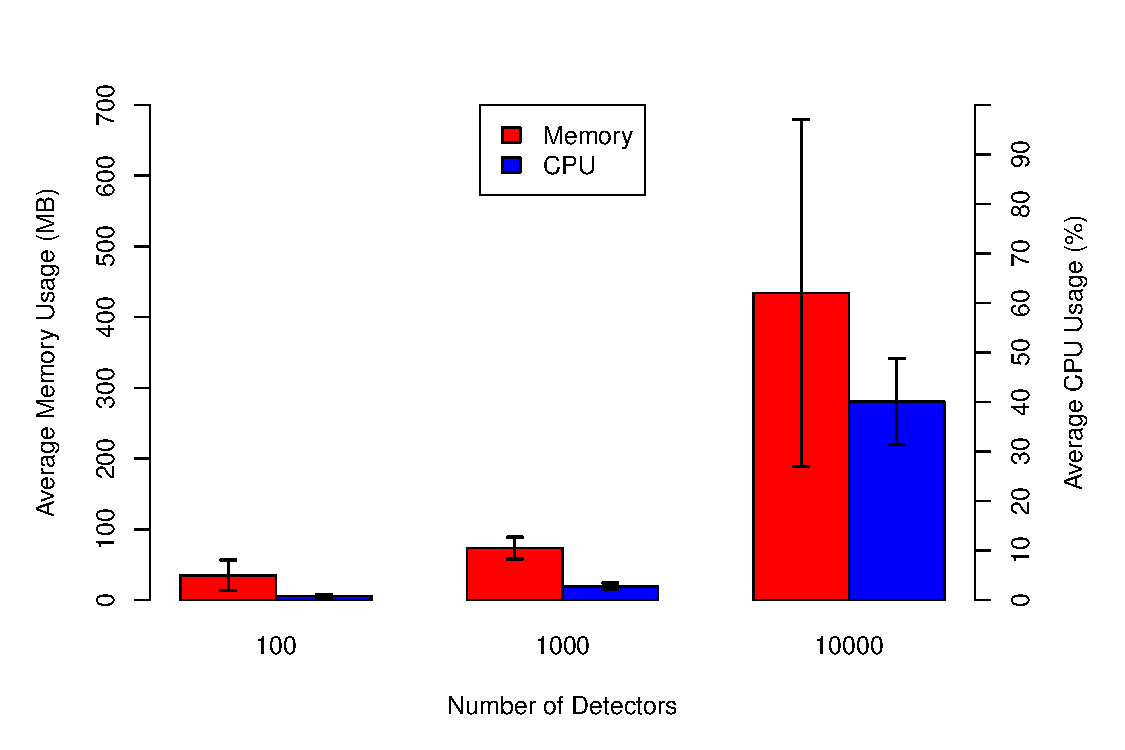
\includegraphics[scale=0.55]{pod_performance}
\caption{Resource utilization of a Roots pod.}
\label{fig:pod_performance}
\end{figure}

Finally, to demonstrate how lightweight and scalable Roots is, we deploy
a Roots pod on a virtual machine with 4 CPU cores and 4GB memory.
To simulate monitoring multiple applications, we run multiple concurrent anomaly
detectors in the pod. Each detector is configured with a 1 hour sliding window.
We vary the number of concurrent
detectors between 100 and 10000, and run each configuration for
2 hours. We track the memory and CPU usage of the
pod during each of these runs using the jstat and pidstat tools. 

Figure~\ref{fig:pod_performance}
illustrates the maximum resource utilization of the Roots pod for different counts of
concurrent anomaly detectors. We see that with 10000 concurrent
detectors, the maximum CPU usage is 238\%, where 400\% is the available limit
for 4 CPU cores. The maximum memory usage in this case is only 778 MB. 
Since each anomaly detector operates with a fixed-sized window, and they
bring additional data into memory only when required, the memory
usage of the Roots pod generally stays low. 
We also experimented with larger concurrent
detector counts, and we were able to pack up to 40000 detectors into the pod before
getting constrained by the CPU capacity of our VM.
This result implies that we can monitor tens of thousands 
of applications using a single pod, thereby scaling up to a very large number
of applications using only a handful of pods.